\section{Introduction}

\begin{figure}[t]
    \centering
    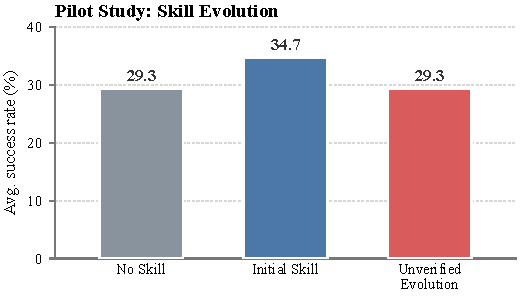
\includegraphics[width=\linewidth]{fig/motivation_unverified_skill_evolution.pdf}
    \caption{\textbf{Pilot study: unverified evolution erases the initial-skill gain.}
    On EB-Habitat, the initial skill raises average success from $29.3\%$ to $34.7\%$, whereas accepting evolved skills without PPO verification returns it to $29.3\%$. Results use Qwen3-VL-8B and the official-protocol-aligned setting with six subsets and 50 episodes per subset.}
    \label{fig:pilot_unverified_evolution}
\end{figure}

Vision-language models (VLMs) have become a general interface for high-level embodied planning, translating natural-language instructions and first-person observations into executable actions. Despite their strong semantic priors, compact open-weight VLMs remain brittle in long-horizon environments, where an agent must preserve object identities across views, distinguish visibility from manipulability, track action-induced state changes, and verify the completion of multiple subgoals. More importantly, an execution failure does not reveal which component is responsible. A failed pickup may indicate a stale visual belief, a missing action precondition, an incorrect procedural skill, or a frozen executor that failed to follow a valid skill. These causes require different learning responses, yet they often produce the same sparse task-level failure signal.

% Vision-Language Models (VLMs) have become a general interface for high-level embodied task planning, translating natural-language instructions and visual observations into executable action sequences. Despite their strong semantic priors, compact open-weight VLMs remain brittle in long-horizon environments. Successful execution requires more than decomposing an instruction: the agent must preserve object identities across views, distinguish visible objects from currently manipulable objects, track action-induced state changes, and verify that every required subgoal has actually been completed. Errors in any of these processes accumulate over long trajectories and frequently lead to repeated invalid actions, instance confusion, and premature termination.

Existing approaches improve embodied agents either by updating model parameters or by externalizing experience into trajectories, reflections, and procedural skills. Non-parametric skill-evolution methods are particularly attractive because they can accumulate reusable execution knowledge while keeping the base model frozen. Skill-Pro, for example, uses semantic gradients and a PPO-inspired gate to generate and validate structured skill revisions, while EmbodiSkill distinguishes reusable skill defects from executor deviations. These methods establish how a skill can be optimized from experience. However, their learning signal remains predominantly trajectory-level: once an episode fails, a language model must infer whether and how the reusable skill should change. Under partial observability, the same failed trajectory is compatible with multiple explanations, so the upstream question remains unresolved: \emph{Does the current experience warrant changing the skill at all?}

% Existing approaches address long-horizon failures from two largely separate directions. Training-based methods encode embodied experience into model parameters through supervised or reinforcement learning, but require substantial data and computation and may still struggle to maintain explicit task state over long interactions. Training-free methods instead store trajectories, reflections, or procedural skills in external memory. In particular, self-evolving skills can accumulate reusable guidance without updating the VLM parameters. However, most textual skills specify what should be done without an explicit mechanism for determining whether the skill is currently visually applicable, whether its next action is executable, or whether its intended effect has been observed.

We refer to the lack of an explicit interface between visual state and procedural execution as the \emph{visual--procedural grounding gap}. Its central learning consequence is a credit-assignment problem. An object being visible does not imply that it is near or pickable; an object missing from the current view does not imply that it is absent; and the absence of an expected visual change does not necessarily imply that the procedure is incorrect. We therefore formulate \emph{visual transition credit assignment}: when a skill-predicted effect disagrees with an evidence-supported belief transition, the agent must determine whether to revise its transient visual belief, persistent action-effect knowledge, reusable procedural skill, or no persistent memory at all. Here, credit assignment refers to assigning a transition mismatch to the component responsible for a persistent update, rather than distributing scalar reward across actions.

Our pilot study exposes why this distinction matters (Fig.~\ref{fig:pilot_unverified_evolution}). With the Qwen3-VL-8B executor frozen, the initial Skill-Pro skill improves average EB-Habitat success from $29.3\%$ to $34.7\%$, but accepting evolved skills without PPO verification erases the gain and returns performance to $29.3\%$. Procedural memory can therefore provide substantial gains, yet an insufficiently verified update can also cause negative transfer. This non-monotonic outcome motivates a mechanism that evaluates not only how a skill should be revised, but whether the evidence supports a persistent revision in the first place.

% We refer to this discrepancy as the visual procedural grounding gap. For example, an object being visible does not imply that it is near or pickable; an object missing from the current view does not imply that it is absent from the environment; and a successful interaction does not automatically guarantee that the updated state is retained in memory. These distinctions are particularly important for multi-instance and long-horizon tasks, in which the agent must bind individual objects to subgoals and preserve their completion status across multiple observations. A procedural skill that ignores such visual evidence can become a source of negative transfer rather than reliable guidance. Our pilot studies support this diagnosis. Although reinforcement-based alignment raises average EB-NAV performance from 0.16 to 0.38, its long-horizon success remains 0.02; moreover, a rigid skill reduces EB-HAB long-horizon success from 0.40 to 0.20, whereas an offline-distilled skill improves success from 0.24 to 0.34 and progress from 0.323 to 0.448. These results suggest that procedural memory is useful only when its applicability and effects are grounded in the evolving visual state. 

Recent work has made progress on both sides of this interface. Multimodal skill methods extract reusable skills and action-level experience from visual interaction trajectories, while state-aware scene graphs maintain dynamic object and interaction states for embodied planning. Symbolic-agent frameworks further refine world models and plans using execution feedback. These advances, however, do not by themselves provide an instance-level criterion for assigning an execution mismatch among transient visual belief, persistent action knowledge, reusable procedural skill, and executor noise. VISTA-Skill focuses on this missing update interface: the graph is not merely an additional planner input, but a shared predicate space in which skill applicability, action preconditions, expected effects, post-action evidence, and termination can be compared.

% Structured visual memory provides a complementary capability. Scene graphs can explicitly represent object instances, spatial relations, functional parts, and interaction states, making them a natural substrate for visual verification. However, existing graph representations are primarily used to support perception, planning, or action feasibility checking, while procedural skill evolution is typically performed directly from trajectory-level textual feedback. Consequently, the visual world model and the procedural memory do not share a common interface: the graph does not specify how a skill should evolve, and the skill does not explicitly predict how the graph should change after execution.


To study this problem, we introduce VISTA-Skill, a training-free framework for evidence-gated procedural skill evolution with a frozen VLM executor. VISTA-Skill maintains an episode interaction graph as an instance-level visual belief and a persistent action-effect graph as reusable, task-independent interaction knowledge. A procedural skill is grounded in the same predicate space through its activation condition, execution and recovery procedure, expected effects, constraints, and termination condition. After each interaction, the system independently derives an evidence-supported belief transition from visual observations and environment feedback and compares it with the transition predicted by the active skill. A hierarchical attribution module first determines whether the mismatch belongs to the episode belief, persistent action model, reusable skill, or no persistent update. Only when a mismatch is repeatedly and confidently attributed to a reusable skill defect does VISTA-Skill identify the affected skill field, generate a constrained patch, and evaluate the candidate on held-out episodes.


% To bridge this gap, we introduce VISTA-Skill, a training-free framework for co-evolving visual interaction graphs and procedural skills. VISTA-Skill maintains two complementary memories: an episode interaction graph that tracks instance-level visual evidence, task progress, and recently verified states, and a persistent action-effect graph that accumulates reusable interaction rules across episodes. A procedural skill is grounded as a set of graph queries and transitions: it specifies when it should be activated, which actions and recovery procedures should be executed, how the graph should be updated after feedback, which graph transition is expected, and when the skill is visually verified as complete. After each interaction, VISTA-Skill compares the expected and observed graph transitions. The resulting graph-skill mismatch determines whether the system should re-observe the scene, repair the graph state, update an interaction rule, preserve a valid skill after an execution lapse, or trigger a reusable skill revision.


Our contributions are three-fold:

\begin{itemize}
  \item We formulate \emph{visual transition credit assignment} for procedural skill evolution under partial observability: given a mismatch between a skill-predicted effect and an evidence-supported belief transition, the agent must identify which memory component, if any, warrants a persistent update. We operationalize this problem through hierarchical attribution labels and update-reliability metrics.
  \item We introduce VISTA-Skill, which represents episode-level visual belief, persistent action-effect knowledge, and reusable procedural skills in a shared graph-predicate space. This interface makes skill activation, action preconditions, expected effects, and termination explicitly verifiable without updating the VLM parameters.
  \item We propose an evidence-gated evolution mechanism that separates transient belief repair, action-model revision, reusable skill patching, and no-update cases. On EB-HAB and EB-NAV, we compare VISTA-Skill primarily with the open-source EmbodiSkill baseline and matched trajectory-level evolution controls using task performance, attribution accuracy, beneficial-update precision, harmful-update rate, and evolution cost.
\end{itemize}

% \begin{itemize}
%   \item We formulate the visual procedural grounding gap in long-horizon embodied agents and introduce a dual-timescale visual interaction graph that separates episode-specific instance states from persistent, reusable action-effect knowledge.
%   \item We propose graph-grounded procedural skills whose activation, state updates, expected effects, and termination are represented as executable graph queries and transitions. This formulation enables structured attribution of perception errors, graph-update errors, interaction-rule conflicts, execution lapses, and skill defects.
%   \item We introduce an evidence-gated, training-free co-evolution mechanism that converts recurring graph-skill mismatches into field-level skill patches and verifies candidate updates before promoting them to a versioned skill pool. We evaluate not only task performance, but also visual-state accuracy, action executability, evolution stability, and teacher-model cost.
% \end{itemize}

